


\subsection{For jet mass}
The general idea of Figure of Merit (FoM) is given in the Appendix; here the InterQuantile range is described since it is used in this note and identical to the one used in the conference BOOST 2016.
The InterQuantile range (IQnR) is here defined as it corresponds to a sigma of a ``perfect'' Gaussian distribution: $q84\%-q16\%$ where $q84\%$ is the 84$^{th}$ percentile and $q16\%$ is the 16$^{th}$, not to be confused with the InterQua\textbf{r}tile Range (IQR) which is the $q75\%-q25\%$ and does not correspond to the sigma. The final descriptor is then divided by the Median ($\iqr$). It provides stability and high sensitivity to left-hand-side and right-hand-side tails.
% The way in which we look at the mass FoM to determine is half of the 68\% of the InterQuantile range (IQnR) (here defined such as it corresponds to a sigma of a ``perfect'' Gaussian distribution: $q84\%-q16\%$ where $q84\%$ is the 84$^{th}$ percentile and $q16\%$ is the 16$^{th}$, not to be confused with the InterQua\textbf{r}tile Range (IQR) which is the $q75\%-q25\%$ and does not correspond to the sigma) divided by the Median ($\iqr$). It provides stability and high sensitivity to left-hand-side and right-hand-side tails.

% Another important FoM, used in literature and in this note, is the response distribution: given the reconstructed mass (calorimeter, track etc.) one can compare it to its $truth$ mass ($m^{truth}$), computed from the particle at MC level before the interaction with the detector:
The IQnR is then applied to the response distribution Figure of Merit: given the reconstructed mass (calorimeter, track etc.) one can compare it to its $truth$ mass ($m^{truth}$), computed from the particle at MC level before the interaction with the detector:

$$R_m=\frac{m^{reco}}{m^{truth}}$$

Standard descriptor of the FoM e.g. in \cite{art35} and here is the $\iqr$ of the $R_m$.
  
  
In Figure \ref{fig:iqrbin} a mass response for a single range of transverse momentum is shown, for the calorimeter mass. On the plot the contours of a standard deviation and of $q16\%$ and $q84\%$ are drawn with dashed and solid lines, respectively, showing the difference induced by the tail. This sort of plot is the key when looking quantitatively to the observable performance and can be found in the Appendix for each of the process studied in every $\pt$ range considered. 
% In this chapter will be shown, however, the quantity which describes this FOM, the IQnR, as a function of $\pt$, in order to get an understanding of the behavior in the entire spectrum and assure the exclusion of local sub-optimalities.

\begin{figure}[!ht]
  \centering
      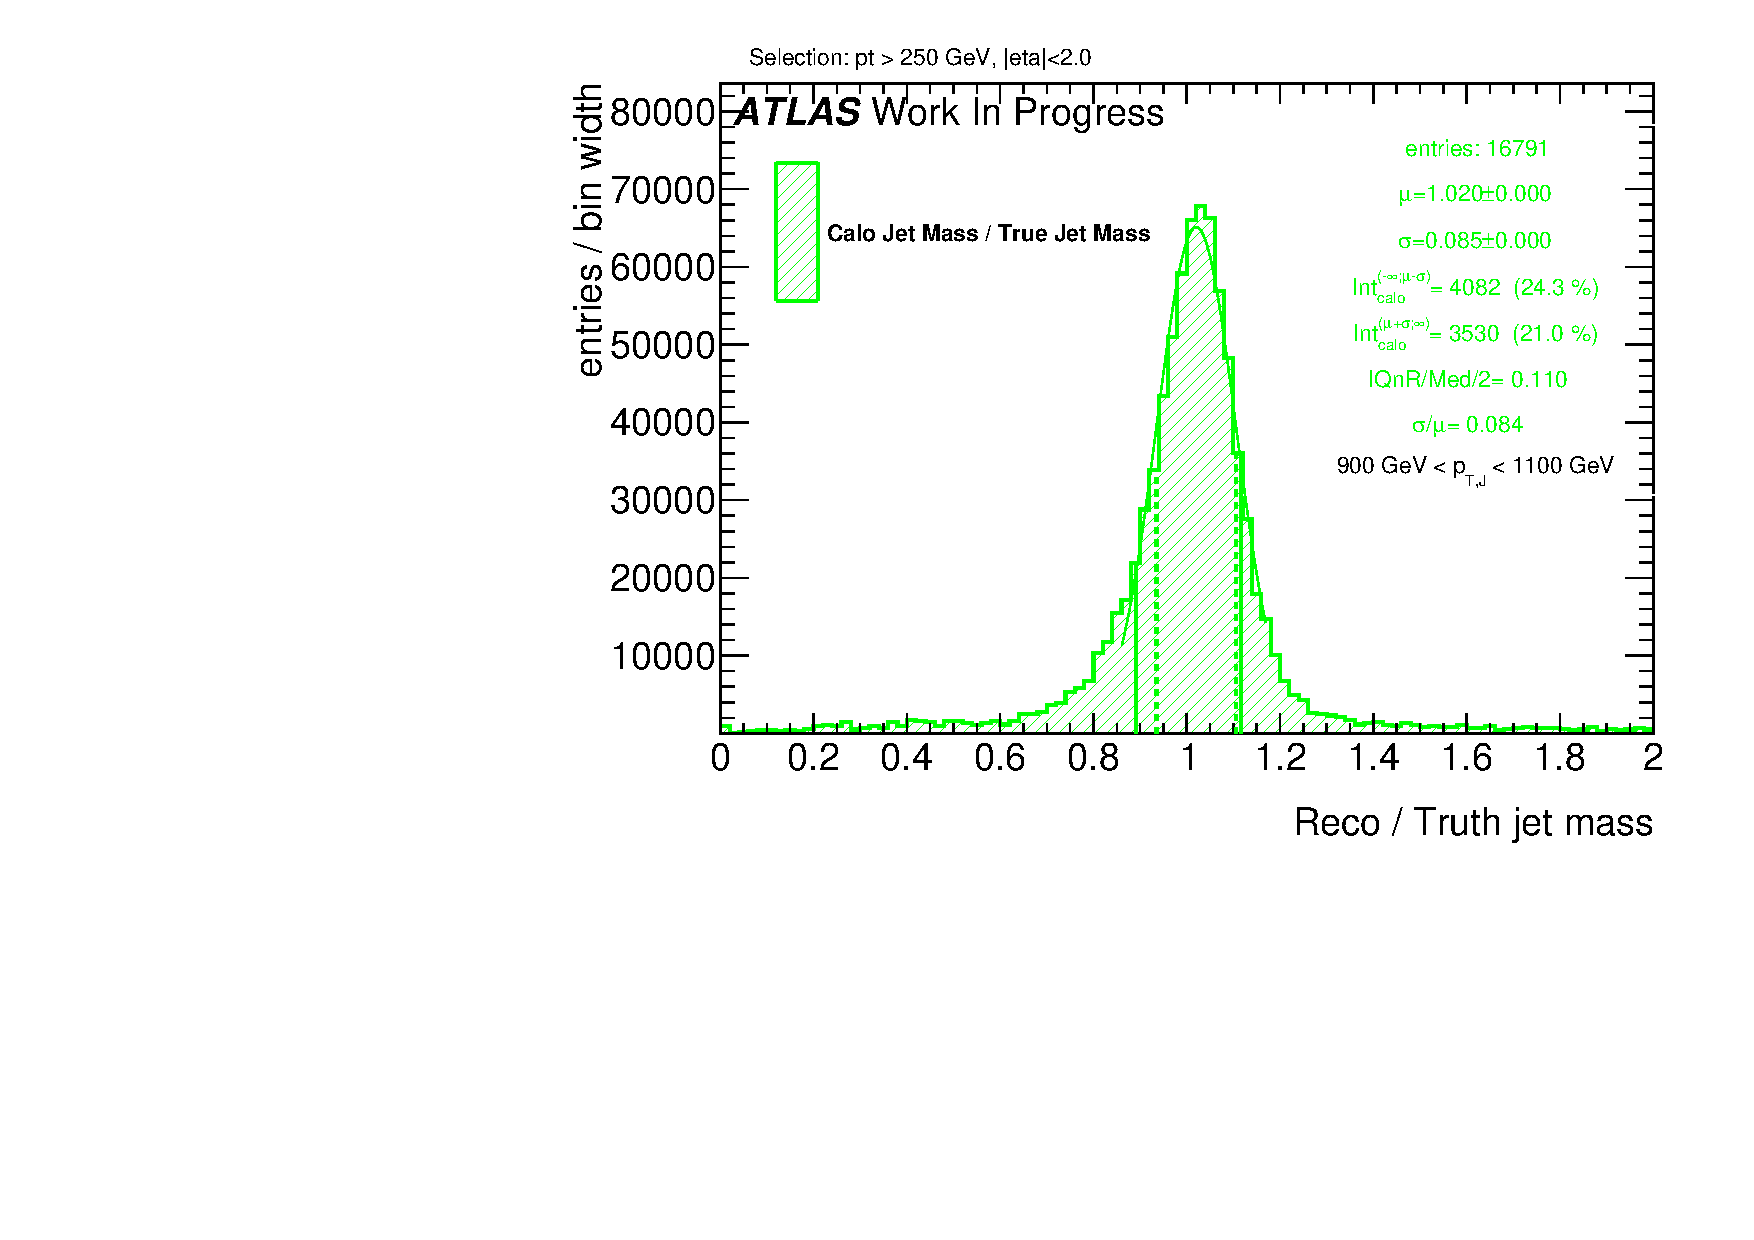
\includegraphics[width=0.7\textwidth]{jet_part/8ResponsePTJ_h_JetRatio_mJ05CALO.pdf}
  \caption[$\mcal$ response single $\pt$ bin]{Calorimeter mass response plot for $W/Z$ jets. One the plot, right, are shown: the number of entries, the mean and the width of the fit to the Gaussian core, the integral from 0 to $\mu-\sigma$ and the one from $\mu+\sigma$ to $+\infty$, the values $\iqr$ and $\sigma/\mu$. On the distribution the dashed vertical lines represent the points $\mu-\sigma$ and $\mu+\sigma$ and the solid lines represent the $q16\%$ and $q84\%$. These lines also explicitly show the asymmetry between the left-hand-side flank, in general more pronounced, and the right-hand-side one}
  \label{fig:iqrbin}
\end{figure}


\subsection{Receiver Operator Characteristics}\label{sec:ROC}
The separation power of discrimination variables can be studied quite intuitively by comparing the signal and background distributions of a certain variable. Another used figure of merit for the performance, especially for comparisons of different variables, is to use \textit{Receiver Operator Characteristics} (ROC) which show the achieved background rejection for different values of signal efficiency (signal fraction left after performing a cut). 
Each point is calculated from the underlying signal and background distributions by integrating the background distribution from zero \footnote[1]{If the signal distribution lies at lower values as the background.} to the point where the desired signal fraction is achieved. The fraction of background events contained in this region are kept when cutting at this signal efficiency, hence the inverse of this fraction, $\frac{1}{\epsilon_{background}}$ is an estimate for the background rejection. The lower the fraction of background events in the region, the better is the achieved exclusion. Accordingly, a good discrimination variable is represented by a ROC with preferably high values of background rejection up to high signal efficiencies.

